%% OxML 2026 Poster Challenge — 2-page extended abstract
%% Track: MLx Health & Bio
%% Submission deadline: 15 May 2026
%% EasyChair: https://easychair.org/conferences/?conf=oxml26

\documentclass[]{ceurart}

\sloppy

\usepackage{listings}
\lstset{breaklines=true}

%% Figure path: works both locally (paper/ → ../figures/) and on Overleaf
%% (figures/ subfolder at project root, or files at root via ./)
\graphicspath{{../figures/}{./figures/}{./}}

\begin{document}

%%
%% Rights management
\copyrightyear{2026}
\copyrightclause{Copyright for this paper by its authors.
  Use permitted under Creative Commons License Attribution 4.0
  International (CC BY 4.0).}

%%
%% Conference information
\conference{OxML 2026 Poster Challenge,
  July 10--18, 2026, Oxford, UK}

%%
%% Title
\title{Where is gout under-treated?
  A global equity analysis using GBD~2023}

%%
%% Author
\author[1]{Yi-Han Cheng}[%
  orcid=0009-0004-5400-1022,
  email=iressa8655@gmail.com,
]
\cormark[1]

\address[1]{Nuffield Department of Orthopaedics, Rheumatology and
  Musculoskeletal Sciences (NDORMS), Botnar Institute for Musculoskeletal
  Sciences, University of Oxford, Oxford, United Kingdom}

\cortext[1]{Corresponding author.}

%%
%% Abstract
\begin{abstract}
Gout is entirely treatable, yet treatment gaps persist across health systems
worldwide. Countries whose gout burden exceeds what their economic development
would predict represent plausible targets for directed public health
investment. We analysed 2021 gout disability-adjusted life year (DALY) rates
from the Global Burden of Disease 2023 study across 166 countries. A baseline
linear regression using log-transformed GDP per capita (purchasing power
parity) established a cross-national benchmark, with residual analysis
identifying countries carrying unexpectedly high burden. A progressive
multimodal regression incorporated population ageing (World Bank 65+
proportion), adult obesity prevalence (WHO Global Health Observatory), alcohol
supply, and dietary meat and seafood supply (FAO Food Balance Sheets 2021).
SHAP (SHapley Additive exPlanations) decomposed feature contributions into
DALY-unit values to enable interpretable cross-variable comparison. Gout DALY
rates varied 20-fold across countries (3.97 to 77.2 per 100,000). GDP alone
explained 38.6\% of cross-national variance (R\textsuperscript{2}~=~0.386).
Population ageing produced the single largest incremental gain
(R\textsuperscript{2}~=~0.476, $\Delta$R\textsuperscript{2}~=~+0.090); SHAP
confirmed ageing as the dominant predictor. Obesity added no independent
explanatory power (R\textsuperscript{2}~=~0.472), reflecting collinearity
with ageing and wealth. The full five-variable dietary model reached
R\textsuperscript{2}~=~0.508. Georgia carried the largest unexplained residual
(+56.9 DALY units above prediction), reduced only marginally by full dietary
adjustment (+51.7), suggesting unmeasured genetic or cultural factors. New
Zealand, Canada, and Australia formed a secondary outlier cluster (+39 to +41
units), consistent with elevated ABCG2 Q141K variant frequency in their
respective Indigenous populations. Cross-national gout inequality is shaped
primarily by population ageing and national wealth. The persistence of the
Anglophone cluster and the Georgia outlier after full adjustment makes a case
for incorporating a genetic modality; UK Biobank data represent the most
suitable resource for this next step.
\end{abstract}

%%
%% Keywords
\begin{keywords}
  global health equity \sep
  gout \sep
  disability-adjusted life years \sep
  GBD 2023 \sep
  multimodal regression \sep
  SHAP \sep
  treatment gap \sep
  residual analysis
\end{keywords}

\maketitle

%%
%% Introduction
\section{Introduction}

Gout affects an estimated 55 million people globally and is the most prevalent
inflammatory arthritis in adults~\cite{gbd2023gout}. It is entirely
manageable with widely available urate-lowering therapy, yet treatment remains
inconsistent across health systems, with diagnosis and initiation of therapy
frequently delayed~\cite{dalbeth2016}. Understanding where burden is highest
relative to national capacity could direct targeted policy and clinical
resource allocation. We address this by combining global burden data with a
progressive multimodal machine learning analysis to identify countries where
gout remains disproportionately under-managed.

%%
%% Methods
\section{Methods}

We extracted 2021 gout DALY rates for 166 countries from the GBD 2023 Results
Tool~\cite{gbd2023gout}. A baseline linear regression (M1) using log-transformed
GDP per capita (purchasing power parity; World Bank~\cite{worldbank}) served as
a cross-national benchmark. Residuals identified countries whose burden
exceeded GDP-predicted levels. A progressive multimodal regression then
incorporated population ageing (World Bank 65+ proportion, M2), adult obesity
prevalence (WHO Global Health Observatory~\cite{who_gho}, M3), alcohol supply
(M4), and dietary meat and seafood supply (FAO Food Balance Sheets
2021~\cite{fao_fbs}, M5). All models were fitted using
scikit-learn~\cite{sklearn}. SHAP~\cite{lundberg2017} decomposed feature
contributions into DALY-unit values for interpretable cross-variable
comparison. Code is available at
\url{https://github.com/Iressa8655/gbd-gout-equity}.

%%
%% Results
\section{Results}

Gout DALY rates varied 20-fold across countries (3.97 to 77.2 per 100,000).
The GDP-only model (M1) explained 38.6\% of cross-national variance. Figure~\ref{fig:main}
illustrates both the regression fit and the countries with the largest positive
residuals. Population ageing yielded the single largest incremental gain (M2:
R\textsuperscript{2}~=~0.476, $\Delta$R\textsuperscript{2}~=~+0.090). SHAP
analysis confirmed ageing as the dominant predictor across all variables
(Figure~\ref{fig:shap}). Obesity contributed no independent explanatory power
(M3: R\textsuperscript{2}~=~0.472), reflecting collinearity with ageing and
wealth. The full five-variable dietary model (M5) reached
R\textsuperscript{2}~=~0.508.

Georgia carried the largest unexplained residual (+56.9 DALY units), which
dietary adjustment reduced only marginally (+51.7 after M5), suggesting
factors beyond those captured by supply-side dietary data. New Zealand, Canada,
and Australia formed a secondary outlier cluster (+39 to +41 units after M5),
consistent with high ABCG2~Q141K frequency in their Indigenous
populations~\cite{phippsgreen2010}.

\begin{figure}[t]
  \centering
  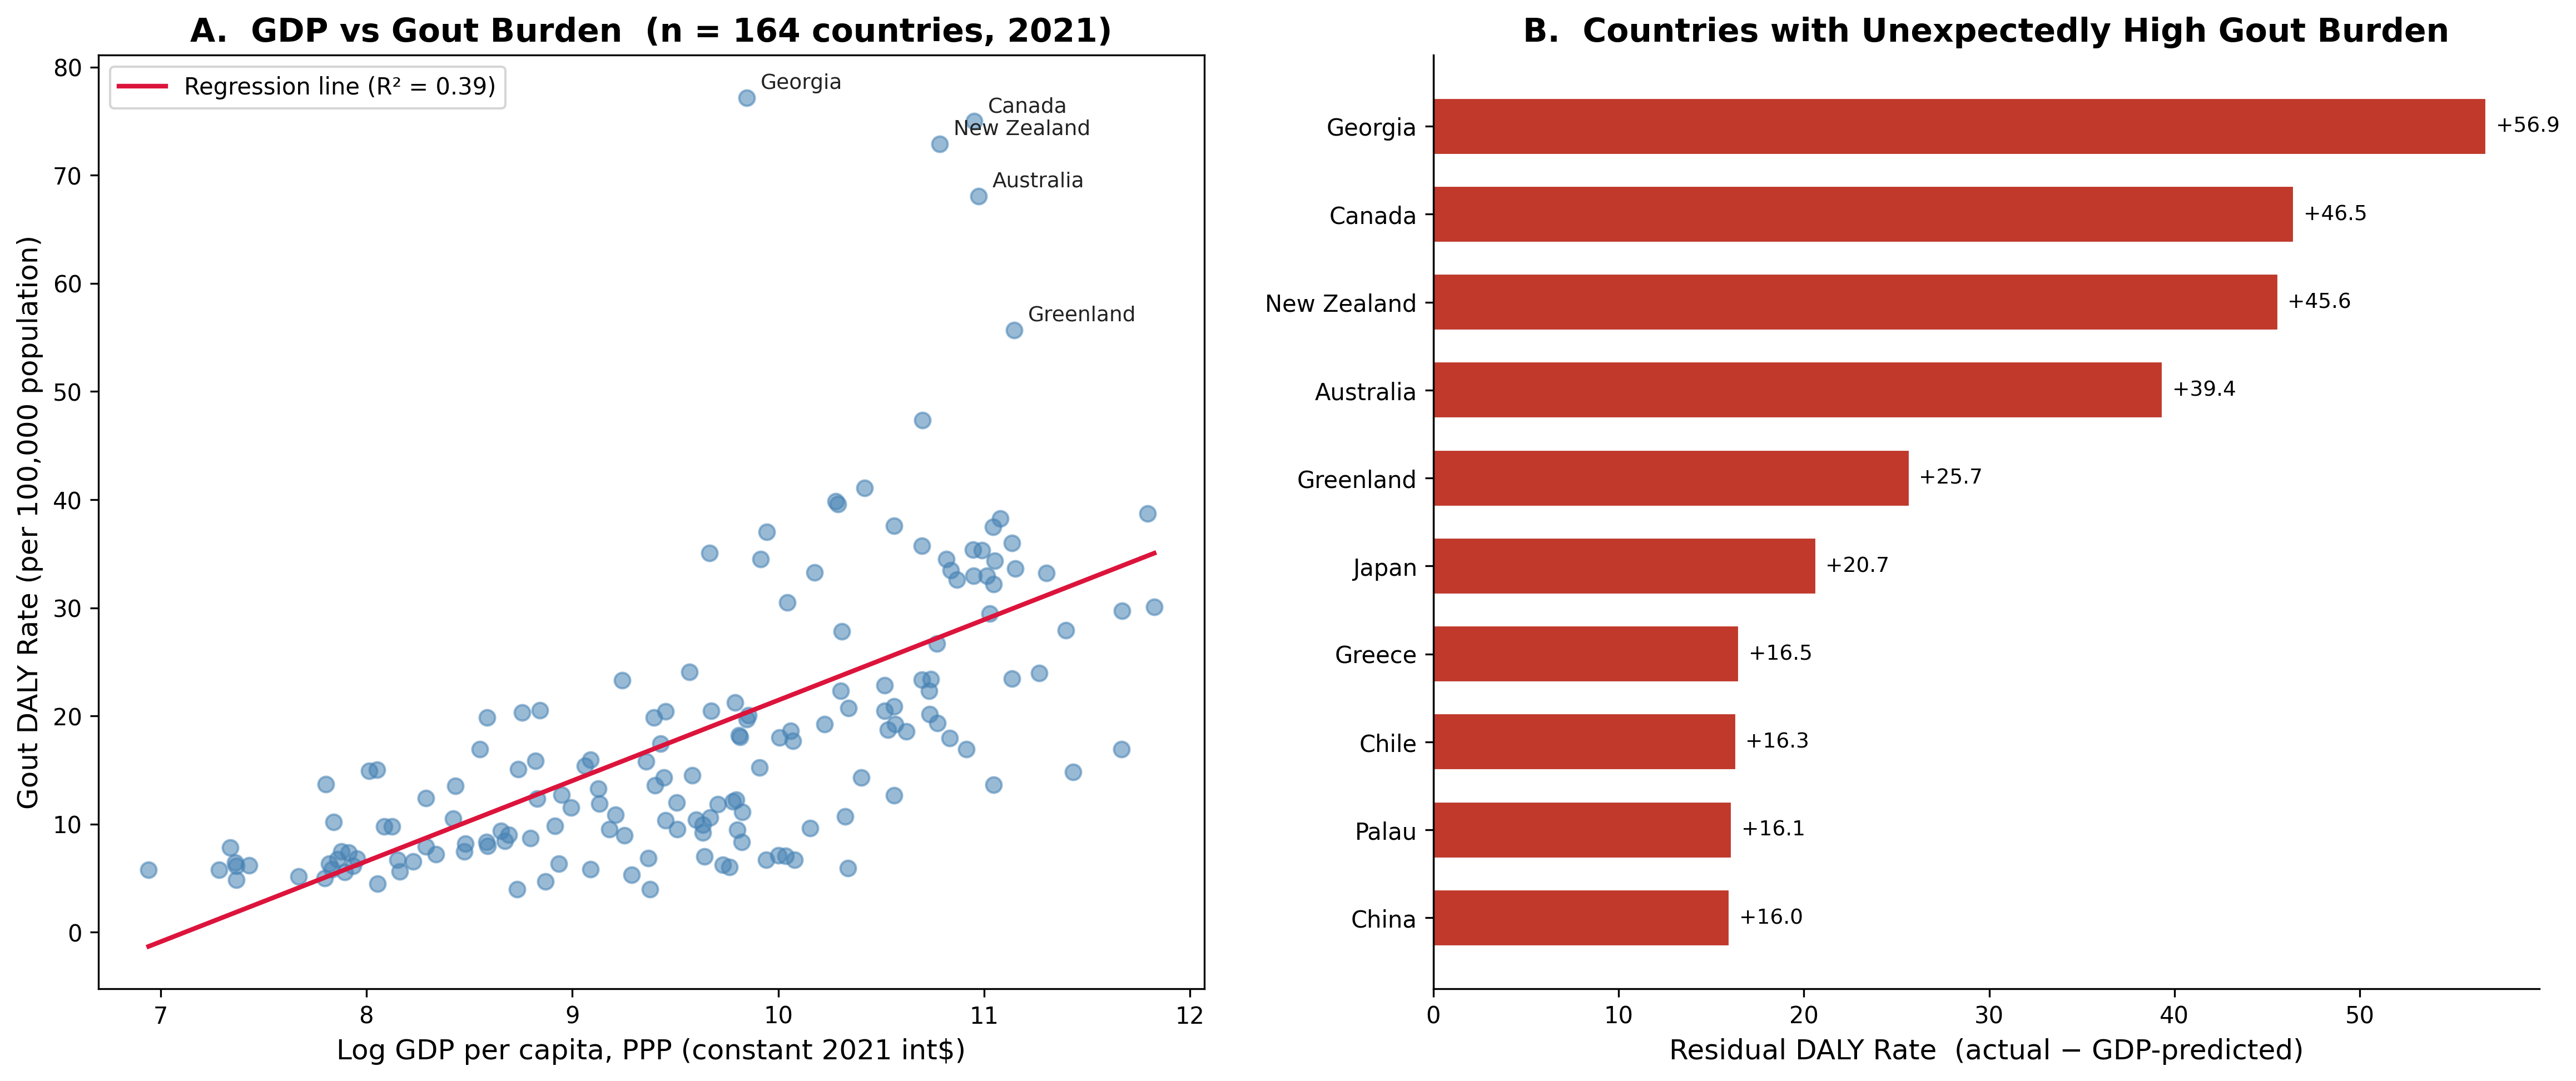
\includegraphics[width=\linewidth]{fig4_dual_panel.png}
  \caption{Left: log GDP per capita versus gout DALY rate across 166 countries
    (R\textsuperscript{2}~=~0.386); the five largest positive residuals are labelled.
    Right: top 10 countries by unexplained residual. Georgia (+56.9) is the
    dominant outlier, followed by an Anglophone cluster.}
  \label{fig:main}
\end{figure}

\begin{figure}[t]
  \centering
  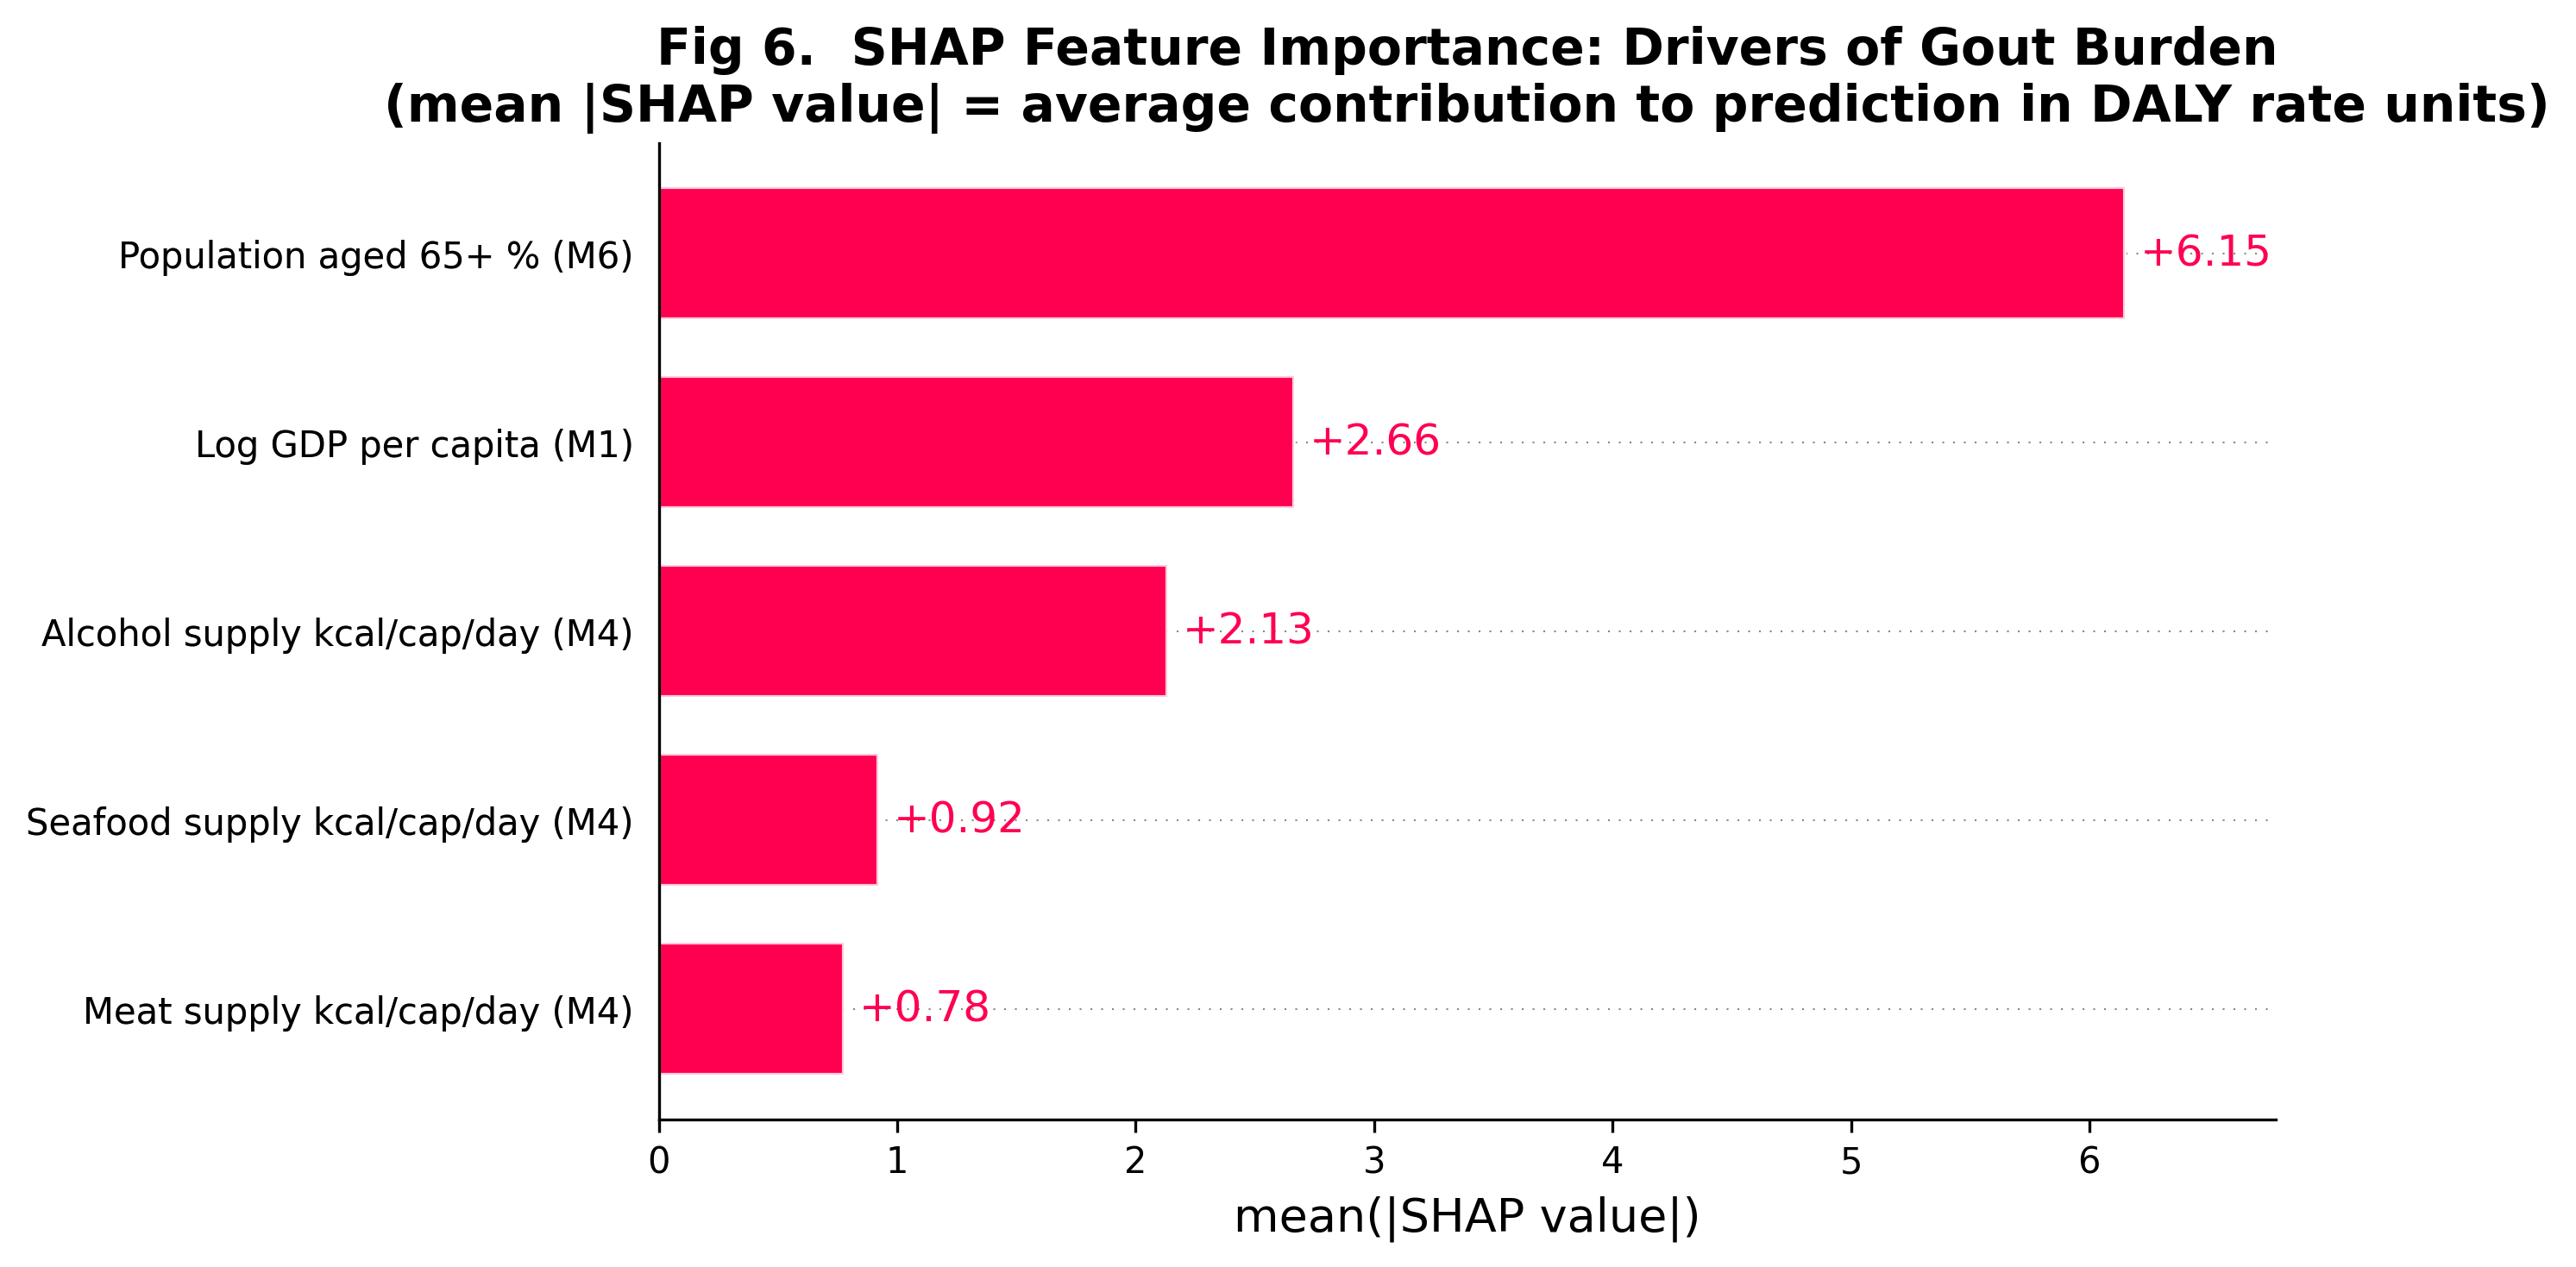
\includegraphics[width=\linewidth]{fig6_shap.png}
  \caption{SHAP feature importance for the five-variable model (M5). Values
    are expressed in DALY rate units, enabling direct comparison across
    variables with differing scales. Population ageing is the dominant
    cross-national predictor.}
  \label{fig:shap}
\end{figure}

%%
%% Conclusion
\section{Conclusion}

Cross-national gout inequality is shaped primarily by population ageing and
national wealth. Dietary supply variables provide modest additional explanatory
power. The persistence of the Anglophone outlier cluster and the Georgia
anomaly after full multimodal adjustment motivates a genetic modality as the
next analytical step. UK Biobank GWAS data for serum urate represent the most
suitable resource for formal validation~\cite{tin2019}.

%%
%% Acknowledgments
\begin{acknowledgments}
The author thanks the GBD 2023 Collaborators for making study data publicly
available via the GBD Results Tool, and the Botnar Institute for
Musculoskeletal Sciences for institutional support.
\end{acknowledgments}

%%
%% Generative AI declaration (required by CEUR-WS from January 2025)
\section*{Declaration on Generative AI}
During the preparation of this work the author used Claude (Anthropic) in
order to assist with Python data processing and figure generation. After using
this tool, the author reviewed and edited the content as needed and takes full
responsibility for the publication's content.

%%
%% Bibliography
\bibliography{oxml26}

\end{document}
